\section{More on Random Variables}
\subsection{Transformation of Random Variables}
Let us consider the problem of determining the distribution functions of random variables that are functions of other random variables. Let $\xi$ be a random variable with distribution function $F_\xi(x)$ (and density $f_\xi(x)$, if it exists), let $\varphi = \varphi(x)$ be a Borel function and $\eta = \varphi(\xi)$. We have
\begin{align}
    F_\eta(y) = \p(\eta \le y) = \p(\xi \in \varphi^{-1}(-\infty, y]) = \int_{\varphi^{-1}(-\infty,y]} \d F_{\xi},
\end{align}
which expresses the distribution function $F_\eta(y)$ in terms of $F_\xi(x)$ and $\varphi$.
\begin{example}
\begin{enumerate}
    \item[]
    \item (Location-scale family) Let $\eta = a\xi + b, \quad a>0$. Then 
    \begin{equation}
        F_\eta (y) = \p(\eta \le y) = \p\bigg(\xi \le \frac{y-b}{a}\bigg) = F_\xi\bigg(\frac{y-b}{a}\bigg).
    \end{equation}
    \item ($\chi^2_1$ distribution) Let $\eta = \xi^2$. Then it is evident that $F_\eta (y) = 0$ if $y<0$. while for $y \ge 0$,
    \begin{align*}
        F_\eta(y) = \p(\xi^2 \le y) &= \p(-\sqrt{y} \le \xi \le \sqrt{y})\\ &= \p_\xi(-\infty, \sqrt{y}] - \p_\xi (-\infty, -\sqrt{y})\\
        &= F_\xi (\sqrt{y}) - F_\xi(-\sqrt{y}) + \p(\xi = -\sqrt{y}).
    \end{align*}
\end{enumerate}
\end{example}

As a further example, let us prove a result that connects the distribution function and probability distribution of a random variable.
\begin{proposition}[Probability Integral Transform] \label{prop:prob_transform}
Let $\xi$ be a random variable on $(\Omega,\F,\p)$ with distribution function $F_\xi(x)$. Let $U$ be a random variable on $([0,1], \B([0,1]), \Leb)$ ($\Leb$ being Lebesgue measure) such that it is uniformly distributed on $[0,1]$ (i.e. $\p_U = \Leb$). Define the right inverse of $F_\xi$ on $[0,1]$:
\begin{equation} \label{eq:right_inverse}
    F^{-1}_\xi(y) = \sup \{ x \,|\, F_\xi(x) < y \}.
\end{equation}
and extend so that $F_\xi(0)=-\infty$ and $F_\xi(1) = \infty$. Then $\xi$ has the same distribution function as $F_\xi^{-1}(U)$. In such case we say $F_\xi^{-1}(U)$ is \textit{equally distributed} as $\xi$, or $\xi \overset{d}{=} F_\xi^{-1}(U)$.
\end{proposition}

\begin{hint}
Let us try to gain a better understanding to the definition of the right inverse: 
\begin{itemize}
    \item To begin, try to verify if $F_\xi$ is strictly increasing (so that $F_\xi(x)$ is a continuous bijection from $(-\infty,\infty)$ to $(0,1)$), then this right inverse of $F_\xi$ agrees with the inverse $F^{-1}_\xi$.
    \item For this special case, we really have
    \begin{align} \label{eq:prob_transform_cts}
        F_{F^{-1}_\xi}(y) = \Leb\bracket{\set{F^{-1}_\xi(U) \le y}} = \Leb\bracket{\set{U \leq F_\xi(y)}} = F_\xi(y)
    \end{align}
    The actual proof won't differ too much.
    \item One can prove a simpler version of this theorem, that the random variable $F_\xi(\xi)$ is equally distributed as $U$.
\end{itemize}
\end{hint}

\begin{proof}
The only caveat of proof is to justify the second equality, that is to prove the equivalence
\begin{equation*}
    F^{-1}_\xi(u) \leq y \iff u \leq F_\xi(y)
\end{equation*}
$(\Leftarrow)$ \textbf{Assume $u \leq F_\xi(y)$.} Then clearly whenever $F_\xi(x) \leq u$ then $F_\xi(x) \leq F_\xi(y) \implies x \in y$, thus clearly $y$ is an upper bound of the set $\set{x \,|\, F_\xi(x) < u}$. \\

$(\Rightarrow)$ \textbf{Assume $F_\xi^{-1}(u) \leq y$ but $u > F_\xi(y)$ by contradiction.} Note in such case we have $y \in \set{x\,|\, F_\xi(x) < u}$, so $y$ is indeed the \textit{maximum} of $\set{x\,|\, F_\xi(x) < u}$. In other words, for any $x > y$ we have $F_\xi(x) \geq u$. Consider an arbitrary monotonic decreasing sequence $(x_n)$ with $x_n > y$ that converges to $y$. We then know that $\lim_{n\to \infty} F_\xi(x_n) = F(y)$ by right continuity, and that $F_\xi(y) \geq u$. This contradicts with our assumption, so we must have $u \leq F_\xi(y)$.
\end{proof}

\begin{example}
Suppose that the distribution function $F$ for $\xi$ uniform on $[0, 1/3] \cup [2/3, 1]$ with an atom at $2/3$. 
\begin{center}
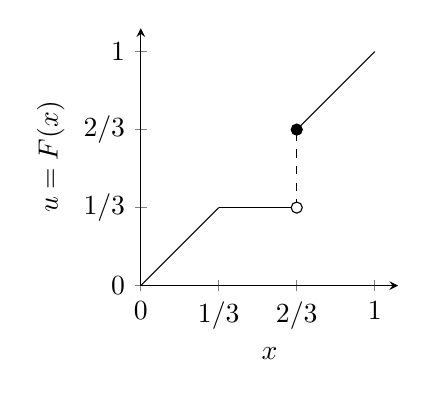
\begin{tikzpicture}
    \begin{axis}[
    axis lines=left,
    xlabel = $x$, ylabel = {$u = F(x)$},
    xmax = 1.1, xtick = {0, 1/3, 2/3, 1}, 
    ymax = 1.1, ytick = {0, 1/3, 2/3, 1},
    xticklabels={$0$, $1/3$, $2/3$, $1$},
    yticklabels={$0$, $1/3$, $2/3$, $1$}, 
    width=0.4\textwidth, height=0.4\textwidth]
    \addplot[domain=0:1/3] {x};
    \addplot[domain=1/3:2/3] {1/3};
    \addplot[domain=2/3:1] {x};
    \addplot[mark=*,only marks] coordinates {(2/3,2/3)};
    \addplot[mark=*,fill=white,only marks] coordinates {(2/3,1/3)};
    \draw [dashed] (2/3,1/3) -- (2/3,2/3);
    \end{axis}
\end{tikzpicture}
\captionof{figure}{An example of distribution function.}
\end{center}
The inverse $F^{-1}(u)$ is shown below
\begin{center}
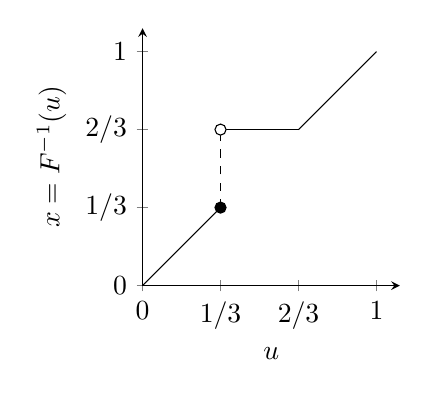
\begin{tikzpicture}
    \begin{axis}[
    axis lines=left,
    xlabel = $u$, ylabel = {$x = F^{-1}(u)$},
    xmax = 1.1, xtick = {0, 1/3, 2/3, 1}, 
    ymax = 1.1, ytick = {0, 1/3, 2/3, 1},
    xticklabels={$0$, $1/3$, $2/3$, $1$},
    yticklabels={$0$, $1/3$, $2/3$, $1$}, 
    width=0.4\textwidth, height=0.4\textwidth]
    \addplot[domain=0:1/3] {x};
    \addplot[domain=1/3:2/3] {2/3};
    \addplot[domain=2/3:1] {x};
    \addplot[mark=*,only marks] coordinates {(1/3,1/3)};
    \addplot[mark=*,fill=white,only marks] coordinates {(1/3,2/3)};
    \draw [dashed] (1/3,1/3) -- (1/3,2/3);
    \end{axis}
\end{tikzpicture}

\captionof{figure}{The psuedo-inverse of the previous example}
\end{center}
\end{example}

Now we turn to the problem of determining $f_\eta(y)$. Let us suppose that the range of $\xi$ is a (finite or infinite) open interval $I = (a,b)$, and that the function $\varphi = \varphi(x)$, with domain $(a,b)$, is continuously differentiable and either strictly increasing or strictly decreasing. We also suppose that $\varphi'(x) \ne 0, x\in I$. Let us write $h(y) = \varphi^{-1}(y)$ and suppose for definiteness that $\varphi$ is strictly increasing. Then when $y \in \varphi(I)$,
\begin{align*}
    F_\eta(y) = \p(\eta \le y) = \p(\varphi(\xi) \le y) = \p(\xi \le \varphi^{-1}(y)) &= \p(\xi \le h(y))
    = \int_{-\infty}^{h(y)}f_\xi(x)\, \d x
    = \int_{-\infty}^y f_\xi(h(z))h'(z)\, \d z.
\end{align*}
Therefore,
\begin{equation}
    f_\eta(y) = f_\xi(h(y))h'(y).
\end{equation}
Similarly, if $\varphi(x)$ is strictly decreasing,
\begin{equation}
    f_\eta(y) = f_\xi(h(y))(-h'(y)).
\end{equation}
Hence in either case
\begin{equation}
    f_\eta(y) = f_\xi(h(y))|h'(y)|.
\end{equation}
\begin{example}
If $\eta = a\xi + b, a\ne 0$, we have
\begin{equation}
    h(y) = \frac{y-b}{a} \quad \text{and} \quad f_\eta(y) = \frac{1}{|a|}f_\xi\bigg(\frac{y-b}{a} \bigg).
\end{equation}
\end{example}
If $\varphi = \varphi(x)$ is neither strictly increasing nor strictly decreasing, the above formula is inapplicable. However, the following generalisation suffices for many applications.
\begin{lemma}
Let $\varphi = \varphi(x)$ be defined on the set $\sum_{k=1}^n[a_k, b_k]$, continuously differentiable and either strictly increasing or strictly decreasing on each open interval $I_k = (a_k, b_k)$, and with $\varphi'(x) \ne 0$ for $x \in I_k$. Let $h_k = h_k(y)$ be the inverse of $\varphi(x)$ for $x \in I_k$, Then
\begin{equation}
    f_\eta(y) = \sum_{k=1}^n f_\xi(h_k(y))|h_k'(y)|\cdot I_{D_k}(y),
\end{equation}
where $D_k$ is the domain of $h_k(y)$.
\end{lemma}
\begin{example}
Let $\eta = \xi^2$ and take $I_1 = (-\infty, 0), I_2 = (0, \infty)$, and find that $h_1(y) = -\sqrt{y}, h_2(y) = \sqrt{y}$, and therefore
\begin{equation}
    f_\eta(y) = 
    \begin{cases}
     \frac{1}{2\sqrt{y}}[f_\xi(\sqrt{y}) + f_\xi(-\sqrt{y})], & y>0,\\
     0, & y\le 0.
    \end{cases}
\end{equation}
In particular, if $\xi \sim N(0,1)$,
\begin{equation}
    f_{\xi^2}(y) = 
    \begin{cases}
     \frac{1}{\sqrt{2\pi y}}e^{-y/2}, & y>0,\\
     0, & y\le 0.
    \end{cases}
\end{equation}
A straightforward calculation shows that
\begin{equation}
    f_{|\xi|}(y) = 
    \begin{cases}
     f_\xi(y) + f_\xi(-y), & y>0,\\
     0, & y\le 0.
    \end{cases}
\end{equation}
\begin{equation}
    f_{\sqrt{|\xi|}}(y) = 
    \begin{cases}
     2y(f_\xi(y^2) + f_\xi(-y^2)), & y>0,\\
     0, & y\le 0.
    \end{cases}
\end{equation}
\end{example}
Let $\xi$ and $\eta$ be random variables with joint distribution $F_{\xi, \eta}(x,y)$, and $\varphi = \varphi(x,y)$ be a Borel function, then 
\begin{equation}
    F_{\varphi(\xi, \eta)} (z) = \int_{\{ x,y: \varphi(x,y) \le z \}} \d F_{\xi,\eta}(x,y).
\end{equation}

\red{Plan: Should we also include some discussion about multivariable transformations?}

\subsection{Independent and Uncorrelated Random Variables}
\subsubsection{Independence}

\begin{definition}[(Mutual) Independence] Let $(\Omega,\F,\p)$ be a measure space.
\begin{itemize}
\item Assume there are events $A_1, A_2, ...$. The finite collection of events $\set{A_1, ..., A_n}$ is independent if $\p\bracket{\cap_{i=1}^n A_n} = \prod_{i=1}^n \p(A_i)$. The infinite collection $\set{A_1,...}$ is (mutually) independent if any finite sub-collections is independent. \\
\item Assume $\F_1, \F_2, ...$ are sub-$\sigma$-algebras of $\F$. Then the collection of sub-$\sigma$-algebras $\set{\F_1, \F_2, ...}$ is mutually independent if for any $A_1 \in \F_1, A_2 \in \F_2, ...$, we have $\p\bracket{\cap_{i=1}^n A_n} = \prod_{i=1}^n \p(A_i)$. The infinite collection $\set{\F_1,...}$ is (mutually) independent if any finite sub-collections is independent.
\item Let $\xi_1, \xi_2, ...$ be random variables on $(\Omega, \F, \p)$. Then the collection $\set{\xi_1, \dots, \xi_n}$ is (mutually) independent if the sub-$\sigma$-algebras $\sigma(\xi_1), ..., \sigma(\xi_n)$ are independent. In particular if $B_1, \dots, B_n \in \B(\R)$, then
\begin{equation*}
    \p(\xi_1 \in B_1,\dots, \xi_n \in B_n) = \prod_{i=1}^n \p(\xi_i \in B_i) = \p_{\xi_i}(B_i).
\end{equation*}
The definition can be extended to the infinite case as above.
\end{itemize}
\end{definition}

\begin{remark}
As seen in elementary probability classes, there is another notion of independence. Let's say there are events $A_1, A_2, ...$, then the collection of events $\set{A_1, ..., A_n}$ is \textit{pairwise} independent if for all $i,j$ with $i \neq j$ we have $\p(A_i \cap A_j) = \p(A_i) \p(A_j)$. It is clear that mutual independence implies pairwise independence but not vice-versa. There are similar notions when considering collections of sub-$\sigma$-algebra or random variables. Note that the notion of mutual independence is far more applicable than the notion of pairwise independence in probability theory. 
\end{remark}

Let us note the following shortcut in establishing mutual independence of sub-$\sigma$-algebra (and hence random variables).

\begin{lemma} \label{lem:independence_shortcut}
Let's say $\F_i = \sigma(\cC_i)$ for some $\pi$-system containing $\Omega$ (that are closed under finite intersection, see theorem \ref{thm:measure_determining}). If we know that for any $C_i \in \cC_i$ (with $\F_i$ belongs to an arbitrary finite sub-collection), $\p(\cap_{i=1}^n C_i) = \prod_{i=1}^n \p(C_i)$, then $\F_1, \F_2,...$ are independent.
\end{lemma}

\begin{proof}
It suffices to consider the case when there are only two $\sigma$-algebra in our collection, denoted as $\set{\F_i := \sigma(\cC_i)}_{i=1,2}$. We break the proof into two steps: 
\begin{itemize}
\item Fix $A \in \cC_1$ and consider the measures $Q_{1,A}(B) := \p(A \cap B)$ and $Q_{2,A}(B) := \p(A) \p(B)$ on $\cC_2$. Since these two measures agree on $\cC_2$, we know from theorem \ref{thm:measure_determining} that for all $A \in \cC_1$ we have $Q_{1,A} = Q_{2,A}$.
\item Now let $B \in \textcolor{blue}{\F_2}$ and consider the measures $\tilde{Q}_{1,B}(A) := \p(B \cap A)$ and $\tilde{Q}_{2,B}(A) := \p(B) \p(A)$. As seen in the above step, these two measures agree on $\cC_2$, so by theorem \ref{thm:measure_determining} we know that for all $B \in \cC_2$ we have $\tilde{Q}_{1,B} = \tilde{Q}_{2,B}$. This completes the proof.
\end{itemize}
\end{proof}

As an immediate corollary, we know that
\begin{corollary}
A necessary and sufficient condition for the random variables $\xi_1, \xi_2, \dots,\xi_n$ to be independent is that
\begin{equation}
    F_\xi(x_1,x_2,\dots,x_n) = F_{\xi_1}(x_1)\dots F_{\xi_n}(x_n)
\end{equation}
for all $(x_1,\dots, x_n)\in \R^n$.
\end{corollary}

\begin{proof}
This comes from the fact that the Borel sets are generated by the collection of left-half-intervals $(-\infty,a]$ and $\R$, with this collection being a $\pi$-system.
\end{proof}

Combining with Fubini-Tonelli theorem, we have
\begin{corollary}
If $\xi = (\xi_1, \dots, \xi_n)$ has a density $f_\xi$, then each $\xi_i$ has a density $f_{\xi_i}$. Furthermore, $\xi_1, \dots, \xi_n$ are independent if and only if 
\begin{equation}
    f_\xi(x_1, x_2, \dots, x_n) = f_{\xi_1}(x_1)\cdots f_{\xi_n}(x_n)
\end{equation}
for all $(x_1, \dots , x_n)$ except possibly for a Borel subset of $\R^n$ with Lebesgue measure zero.
\end{corollary}

\begin{corollary}
If $\xi_1,\dots, \xi_n$ are independent and $\xi_i$ has density $f_{\xi_i}$, $i = 1,\dots, n$, then $\xi$ has a density $f_\xi$ given by
\begin{equation*}
    f_\xi(x_1, x_2, \dots, x_n) = f_{\xi_1}(x_1)\cdots f_{\xi_n}(x_n).
\end{equation*}
\end{corollary}

\begin{remark}
Note that if $\xi_1,\dots, \xi_n$ each have a density, it does not follow that $(\xi_1,\dots, \xi_n)$ has a density.
\end{remark}

\subsubsection{Convolution of Independent Random Variables}
Let $\xi, \eta$ be two independent random variables, so $F_{(\xi,\eta)} (x,y)= F_\xi(x) F_\eta(y)$. Consider the random variable $\xi + \eta$. We get
\begin{align*}
    F_{(\xi,\eta)}(z) &= \int_{\{x,y:x+y \le z \}} \d F_\xi(x) \cdot \d F_\eta(y)\\
    &=\int_{\R^2}\chi_{x+y\le z} \, \d F_\xi(x) \cdot \d F_\eta(y)\\
    &=\int_{-\infty}^\infty \, \d F_\xi(x) \bigg\{ \int_{-\infty}^\infty \chi_{x+y \le z} \, \d F_\eta(y) \bigg\}\\
    &=\int_{-\infty}^\infty F_{\eta}(z-x) \, \d F_\xi(x)
\end{align*}

and similarly 
\begin{equation*}
    F_{(\xi,\eta)}(z) = \int_{-\infty}^\infty F_{\xi}(z-y) \d F_\eta(y).
\end{equation*}

Thus we obtained the following result
\begin{proposition}
The distribution function $F_{\xi + \eta}$ of the sum of two independent random variables is the convolution of their distribution functions. 
\begin{equation}
    F_{(\xi,\eta)}(z) = F_\xi * F_\eta = \int_{-\infty}^\infty F_{\xi}(z-y) \d F_\eta(y) = \int_{-\infty}^\infty F_{\eta}(z-x) \d F_\xi(x).
\end{equation}
\end{proposition}

Similarly, we can easily obtain
\begin{corollary}
If $\xi, \eta$ are independent a.c. random variables, then the density $f_{\xi + \eta}$ is the convolution of the densities.
\begin{equation}
    f_{\xi + \eta} = f_\xi * f_\eta = \int_{-\infty}^\infty f_{\xi}(z-y) f_\eta(y) \d y = \int_{-\infty}^\infty f_{\eta}(z-x) f_\xi(x)\d x.
\end{equation}
\end{corollary}

\begin{example}[$\xi, \eta$ - independent a.c. random variables]
\begin{itemize}
    \item[]
    \item Let $\xi \sim N(m_1,\sigma_1^2)$ and $\eta \sim N(m_2,\sigma_2^2)$, i.e.
    \begin{equation*}
        f_\xi(x) = \frac{1}{\sigma_1}\varphi\bigg(\frac{x-m_1}{\sigma_1} \bigg), \quad f_\eta(x) = \frac{1}{\sigma_2}\varphi\bigg(\frac{x-m_2}{\sigma_2} \bigg),
    \end{equation*}
    where
    \begin{equation*}
        \varphi(x) = \frac{1}{\sqrt{2\pi}}e^{-x^2/2}.
    \end{equation*}
    Then
    \begin{equation*}
        f_{\xi + \eta}(z) = \int_{-\infty}^\infty f_{\eta}(z-x)f_\xi(x)\d x = \frac{1}{\sqrt{\sigma_1^2 + \sigma_2^2}}\varphi \bigg( \frac{z - (m_1 + m_2)}{\sqrt{\sigma_1^2+\sigma_2^2}} \bigg).
    \end{equation*}
    Thus the sum of two independent normal random variables is the normal random variable $N(m_1 + m_2, \sigma_1^2 + \sigma_2^2)$. 
    \item Let $\xi_1, \xi_2, \dots \xi_n$ be independent $N(0,1)$. Then
    \begin{equation*}
        f_{\xi_1^2 + \cdots + \xi_n^2}(x) = 
        \begin{cases}
         \frac{1}{2^{n/2}\Gamma(n/2)}x^{(n/2)-1}e^{-x/2}, & x>0,\\
         0, &x\le 0.
        \end{cases}
    \end{equation*}
    The random variable $\xi_1^2 + \cdots + \xi_n^2$ is usually denoted by $\chi_n^2$ and its distribution is the $\chi^2$-distribution with $n$ degrees of freedom.
\end{itemize}
\end{example}

\begin{proposition}
Let $\xi$ and $\eta$ be independent random variables with $\E[\xi]<\infty$, $\E[\eta] < \infty$. Then $\E[\xi \eta] < \infty$ and $\E[\xi \eta] = \E[\xi] \E[\eta]$.
\end{proposition}

\begin{proof}
We utilise the four-step proofs. First assume $\xi, \eta \ge 0$. Consider
\begin{equation*}
    \xi_n = \sum_{k=0}^\infty \frac{k}{n}\chi_{\{\frac{k}{n} \le \xi(\omega) < \frac{k+1}{n}\}},
\end{equation*}
\begin{equation*}
    \eta_n = \sum_{k=0}^\infty \frac{k}{n}\chi_{\{\frac{k}{n} \le \eta(\omega) < \frac{k+1}{n}\}}.
\end{equation*}
Then $\xi_n \le \xi, \eta_n \le \eta$, $|\xi - \xi_n|\le \frac{1}{n}, |\eta - \eta_n|\le \frac{1}{n}$ for all $n$. Since $\xi, \eta$ are integrable, by dominated convergence theorem
\begin{equation*}
    \lim_{n\rightarrow \infty} \E[\xi_n] = \E[\xi], \quad \lim_{n\rightarrow \infty} \E[\eta_n] = \E[\eta].
\end{equation*}
Now write
\begin{align*}
    \E[\xi_n \eta_n] &= \sum_{i,j \ge 0} \frac{jk}{n^2}\E[\chi_{\{ \frac{j}{n} \le \xi < \frac{j+1}{n}\}} \chi_{\{ \frac{k}{n} \le \eta < \frac{k+1}{n}\}}] \quad \text{(Monotone Convergence)}\\
    &= \sum_{i,j \ge 0} \frac{jk}{n^2} \E[\chi_{\{ \frac{j}{n} \le \xi < \frac{j+1}{n}\}}] \E[\chi_{\{ \frac{k}{n} \le \eta < \frac{k+1}{n}\}}]  \quad \text{(Independence)}\\
    &=\E[\xi_n]\E[\eta_n]
\end{align*}
Since 
\begin{equation*}
    |\E[\xi\eta]-\E[\xi_n \eta_n]| \le \E[|\xi \eta - \xi_n \eta_n|] = \E[|\xi(\eta - \eta_n)+ \eta_n(\xi - \xi_n)|] \le \frac{1}{n}\E[|\xi|]+\frac{1}{n}\E\bigg[|\eta|+\frac{1}{n}\bigg] \rightarrow 0
\end{equation*}
as $n \rightarrow \infty$, we have that
\begin{equation*}
    \E[\xi \eta] = \lim_{n \rightarrow \infty} \E[\xi_n \eta_n] = \lim_{n \rightarrow \infty} \E[\xi_n] \lim_{n \rightarrow \infty}\E[\eta_n] = \E[\xi] \E[\eta],
\end{equation*}
and $\E[\xi \eta] < \infty$. The result in the general case follows by using the representation $$\xi = \xi^+ - \xi^-, \eta = \eta^+ - \eta^-.$$
\end{proof}

In fact, we can prove a stronger converse
\begin{proposition} \label{prop:independence_by_product}
Under the above setting, $\xi,\eta$ are independent iff for all Borel-measurable functions $f,g$ we have $\E[f(\xi) g(\eta)] = \E[f(\xi)] \E[g(\eta)]$.
\end{proposition}

\begin{hint}
For $(\Leftarrow)$ we directly apply the assumption for $f = \chi_{A_1}, g = \chi_{A_2}$, such that $A_1 = \xi_1^{-1}(B_1)$ for an arbitrary $B_1 \in \B(\R)$ and similarly for $A_2$. For $(\Rightarrow)$ we utilise the four-step proof similar to above.
\end{hint}

\subsubsection{Correlation}
We also define another notion of "unrelatedness" of two random variables. First we define the notion of \textbf{covariance}:

\begin{definition}[Covariance]
Let $\xi, \eta$ be a pair of random variables on the same probability space. Their \textbf{covariance} is
\begin{equation}
    \cov[\xi, \eta] := \E[(\xi - \E[\xi])(\eta - \E[\eta])].
\end{equation}
if the expectation above exists.
\end{definition}
\begin{remark}
Note that 
\begin{equation*}
    \V[\xi + \eta] = \V[\xi] + \V[\eta] + 2\cov[\xi, \eta],
\end{equation*}
so 
\begin{equation*}
    \cov[\xi, \eta] = 0 \implies \V[\xi + \eta] = \V[\xi] + \V[\eta].
\end{equation*}
\end{remark}

\begin{definition}[Uncorrelated variables]
The random variables $\xi$ and $\eta$ are called \textbf{uncorrelated} if $$\cov[\xi, \eta] = 0.$$
\end{definition}

\begin{corollary} \label{cor:independence_uncorrelated}
Independent random variables are uncorrelated.
\end{corollary}
\begin{proof}
Indeed, using the theorem from above,
\begin{equation*}
    \cov[\xi, \eta] = \E[\xi \eta] - \E[\xi]\E[\eta] = 0.
\end{equation*}
\end{proof}
The converse is not true. 

\begin{example}
    Consider for example the random variable $\alpha$ which takes the values $0,\frac{\pi}{2}, \pi$ with probability $\frac13$. Then $\xi = \sin{\alpha}, \eta = \cos{\alpha}$ are uncorrelated ($\E[\xi] = \frac13, \E[\eta] = 0$), but they are not independent since
    \begin{equation*}
        \p(\xi = 1, \eta = 1) = 0 \ne \frac19 = \p(\xi = 1)\p(\eta = 1).
    \end{equation*}
    Indeed we can also see that the random variables $\xi, \eta^2$ are correlated, since $\E[\eta^2] = 2/3$ and $\E[\xi] \E[\eta+1] = 2/9$, but $\cov[\xi, \eta^2] = -2/9$.
\end{example}

% might add some remarks on independence of moments
\newpage